\section{Mô phỏng với proteus}
Để kiểm tra và đánh giá hoạt động của hệ thống điều khiển đèn giao thông, nhóm đã sử dụng phần mềm \textbf{Proteus} để mô phỏng toàn bộ mạch điện và chương trình điều khiển. Mô phỏng giúp phát hiện các lỗi logic, kiểm tra chính xác thứ tự hoạt động của các đèn và đảm bảo hệ thống vận hành đúng như thiết kế trước khi triển khai thực tế. \\

Mục tiêu mô phỏng:
\begin{itemize}
    \item Xác thực logic điều khiển trong từng chế độ hoạt động.
    \item Đảm bảo đèn giao thông chuyển pha đúng thứ tự và đúng thời gian.
    \item Kiểm tra hiển thị trên LCD và LED 7 đoạn có hoạt động chính xác hay không.
    \item Kiểm tra tín hiệu từ các nút nhấn có được vi điều khiển nhận đúng không.
\end{itemize}
\subsection{Mô phỏng chế độ tự động}
\begin{figure}[H]
    \centering
    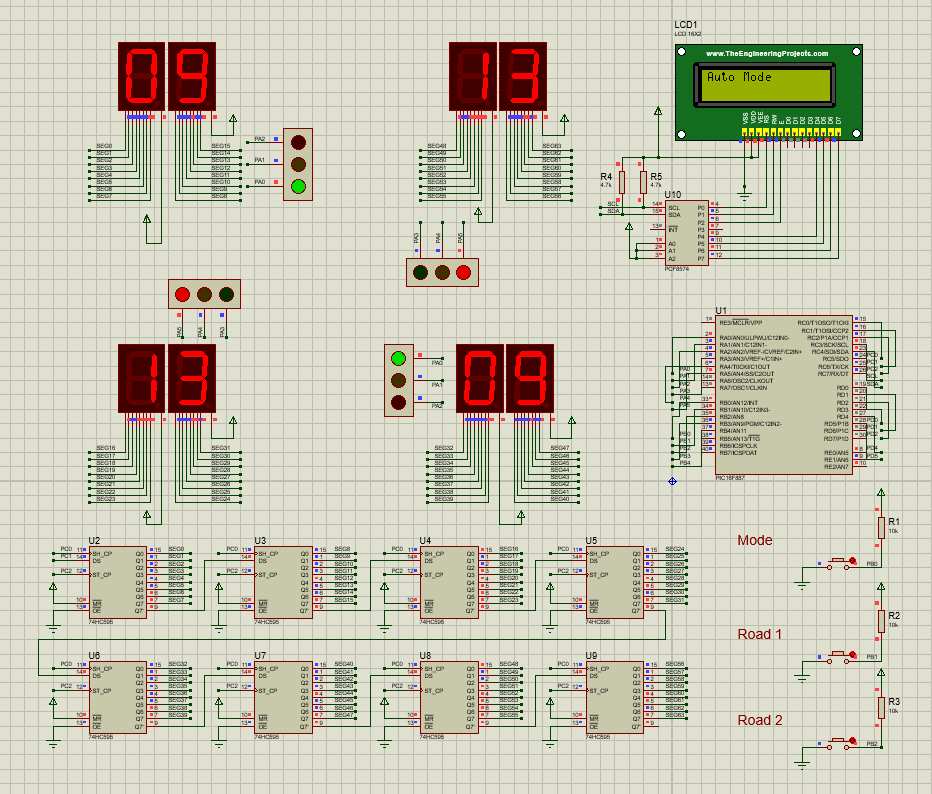
\includegraphics[width=0.7\textwidth]{pictures/autoproteus.png}
    \caption{Mô phỏng chế độ tự động với Proteus}
\end{figure}
Khi bắt đầu mô phỏng, hệ thống khởi động ở chế độ mặc định là \textbf{AUTO MODE}. LCD hiển thị dòng chữ “AUTO MODE”. Các cụm đèn giao thông hoạt động tuần tự theo 4 pha chính:
\begin{enumerate}
    \item Đèn đỏ hướng 1 (R1) sáng, đèn xanh hướng 2 (G2) sáng, đếm ngược.
    \item Đèn đỏ hướng 1 (R1) sáng, đèn vàng hướng 2 (Y2) sáng, đếm ngược.
    \item Đèn xanh hướng 1 (G1) sáng, đèn đỏ hướng 2 (R2) sáng, đếm ngược.
    \item Đèn vàng hướng 1 (Y1) sáng, đèn đỏ hướng 2 (R2) sáng, đếm ngược.
\end{enumerate}
Các LED 7 đoạn hiển thị thời gian đếm ngược tương ứng với từng pha.

\subsection{Mô phỏng chế độ thủ công}
\begin{figure}[H]
    \centering
    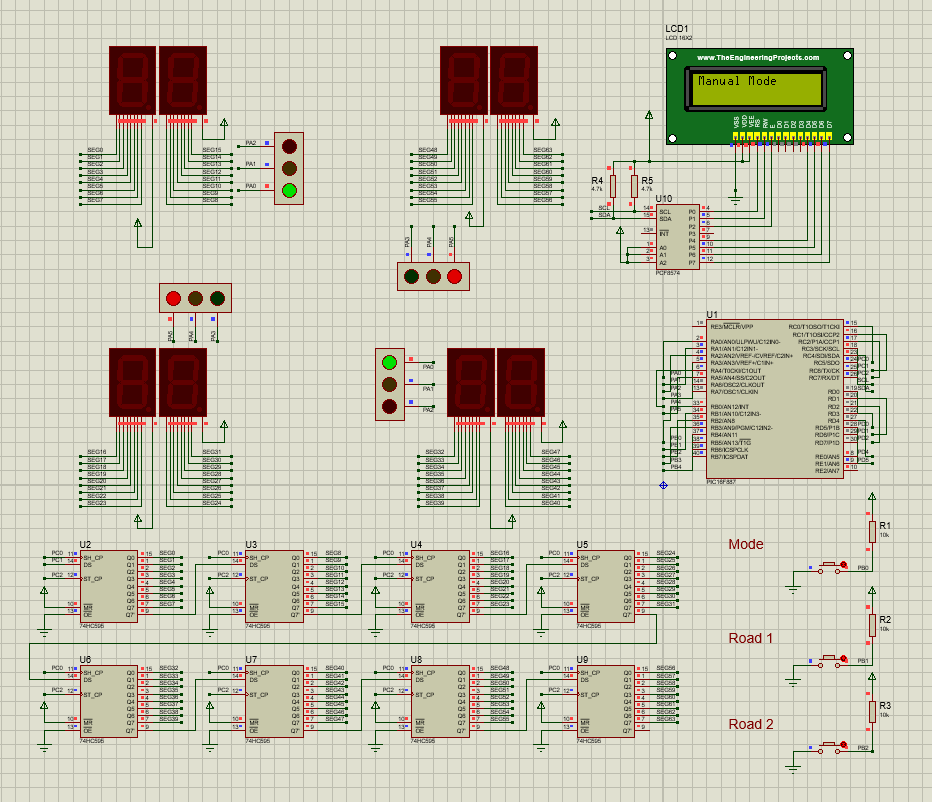
\includegraphics[width=0.7\textwidth]{pictures/manualproteus.png}
    \caption{Mô phỏng chế độ thủ công với Proteus}
\end{figure}
Khi nhấn nút MODE, hệ thống chuyển sang \textbf{MANUAL MODE}, LCD cập nhật dòng chữ tương ứng. Ở chế độ này:
\begin{itemize}
    \item Người dùng nhấn \texttt{BUTTON1} để chuyển từ pha R1-G2 sang G1-R2.
    \item Nhấn \texttt{BUTTON2} để chuyển từ G1-R2 sang Y1-R2.
    \item Sau đó hệ thống quay lại pha đầu tiên.
\end{itemize}
Trong mô phỏng, trạng thái đèn chỉ thay đổi khi có thao tác từ người dùng, giúp kiểm soát giao thông linh hoạt trong tình huống đặc biệt.


\subsection{Mô phỏng chế độ ban đêm}
\begin{figure}[H]
    \centering
    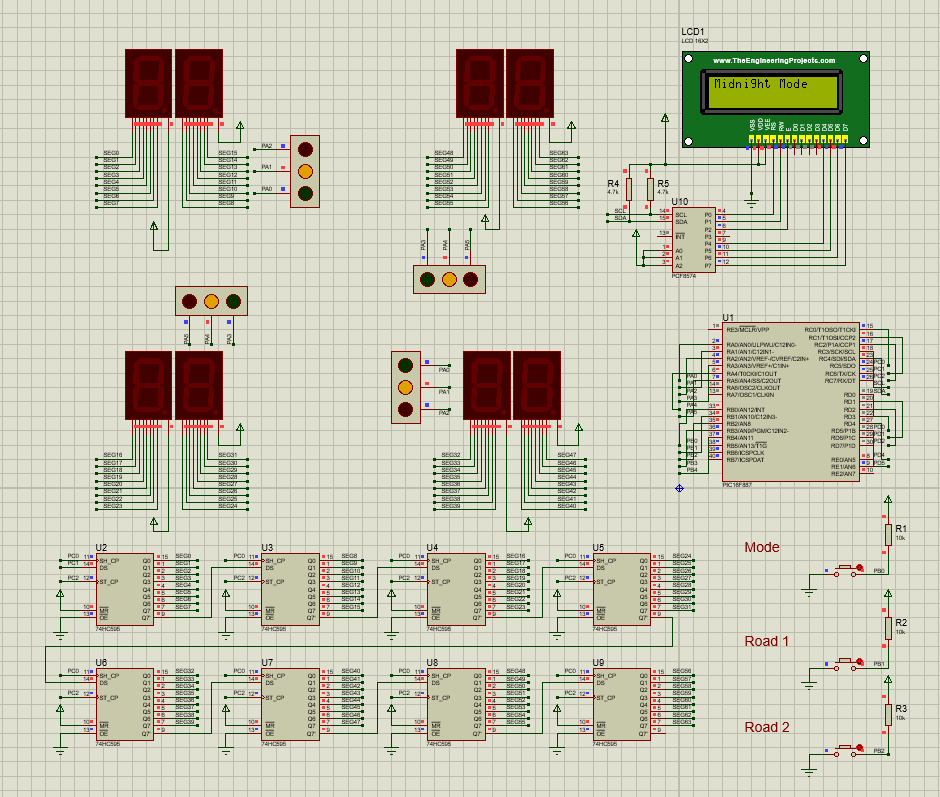
\includegraphics[width=0.7\textwidth]{pictures/nightproteus.png}
    \caption{Mô phỏng chế độ ban đêm với Proteus}
\end{figure}
Khi nhấn MODE lần nữa, hệ thống chuyển sang \textbf{NIGHT MODE}. LCD hiển thị “NIGHT MODE”. Tất cả đèn giao thông sẽ tắt, chỉ còn đèn vàng (Y1, Y2) của hai hướng nhấp nháy liên tục để cảnh báo. Điều này được thể hiện rõ trong mô phỏng bằng hiệu ứng bật/tắt liên tục với chu kỳ đều đặn.
\subsection{Nhận xét và đánh giá}
\begin{itemize}
    \item Các chế độ hoạt động đúng như thiết kế và chương trình đã lập trình.
    \item Đèn giao thông chuyển pha chính xác, không có tình trạng xung đột tín hiệu.
    \item LCD và LED 7 đoạn hoạt động ổn định, hiển thị đúng nội dung.
    \item Việc sử dụng Proteus giúp nhóm tiết kiệm thời gian thử nghiệm phần cứng, đồng thời kiểm tra logic chương trình một cách trực quan và hiệu quả.
\end{itemize}
$\Rightarrow$ Tiến hành xây dựng phần cứng thực tế.
\cleardoublepage